\graphicspath{{./Figs/}}

\chapter{Introduction} 
\label{sec:Background}

% What is a MAV

% These advances have largely been brought about by technological advances in power processors, miniature sensors, and control theory \cite{NONAMI2007}.


Unmanned aerial vehicles (UAVs) are used throughout various industries to conduct missions that are either dangerous, difficult or tedious for humans to perform. Recently UAVs have seen unprecedented growth for both commercial \cite{Liu2014} and military \cite{Chaturvedi2019} \cite{Fan2018} use. The capability to fly within narrow spaces gives Micro Aerial Vehicles (MAVs) a significant advantage over general UAVs in specific use cases. MAVs, in particular, are more manoeuvrable in cluttered environments, such as, collapsed buildings, commercial centres, and search and rescue missions. Given current technology, MAVs could provide coordinates of trapped victims in areas where it would be dangerous to search manually  \cite{Valavanis2007}. Possible applications of MAVs include dangerous gas detection, environmental monitoring, border patrol, mapping, precision agriculture, homeland security, and drug interdiction \cite{Liu2014} \cite{Valavanis2007}. MAVs ability to be much quieter and concealed give it a major advantage over UAVs.


Today defence programs around the world utilize UAVs for reconnaissance, surveillance, damage assessments, and communication relay \cite{Chaturvedi2019} \cite{Fan2018} \cite{Valavanis2007}. Miniature aerial vehicles (MAVs) have even more recently seen major research interest, particularly in the last decade \cite{Valavanis2007}.  The relative size of MAVs to other typical aircraft is shown in Figure \ref{fig:sizes}. Smaller vehicles are intended to lower the total cost of systems currently used and increase the portability of MAVs \cite{Stephen2022}. The most limiting factors holding back MAVs from being more predominantly used, are propulsion, configuration, and flight control issues \cite{Stephen2022}.


\begin{figure}[H]
  \centering
%   \hspace*{-0.4cm}
   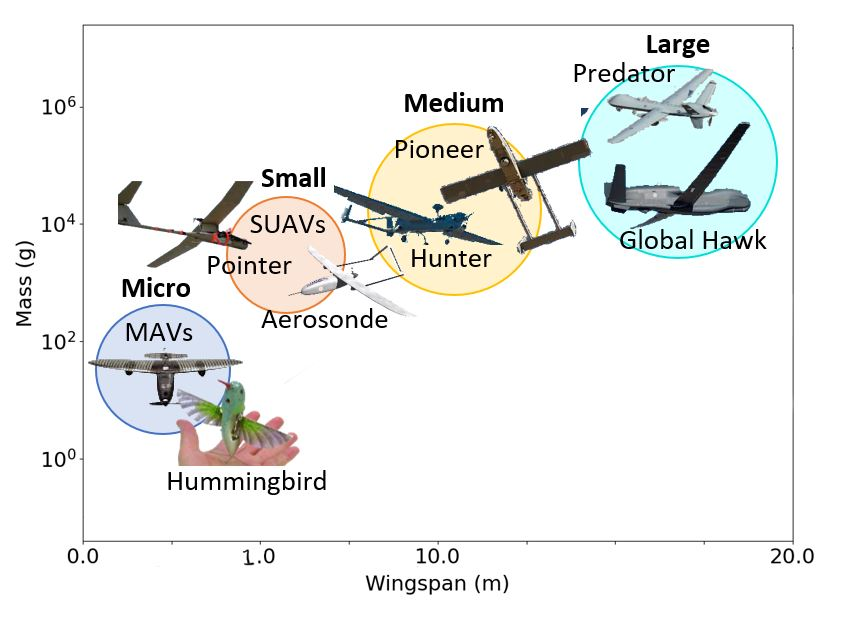
\includegraphics[width=\linewidth]{01_Introduction/Figs/replacement.JPG}
  \caption{MAV gross weight with wing span. Figure is adapted \cite{uavsize}. Image sources: \cite{MAVImage} \cite{Hummingbird} \cite{Ava} \cite{Aerosonde} \cite{hunter} \cite{pioneer} \cite{MQ9} \cite{hawk}}
  \label{fig:sizes}
\end{figure}


MAVs fall into three main categories. These are fixed wings \cite{Stanford2008}, rotary wings \cite{Lasek2001} and flapping wings \cite{Platzer2012}, which can also be used in combination.







\begin{figure}[H]
     \centering
     \begin{subfigure}[b]{0.3\textwidth}
         \centering
         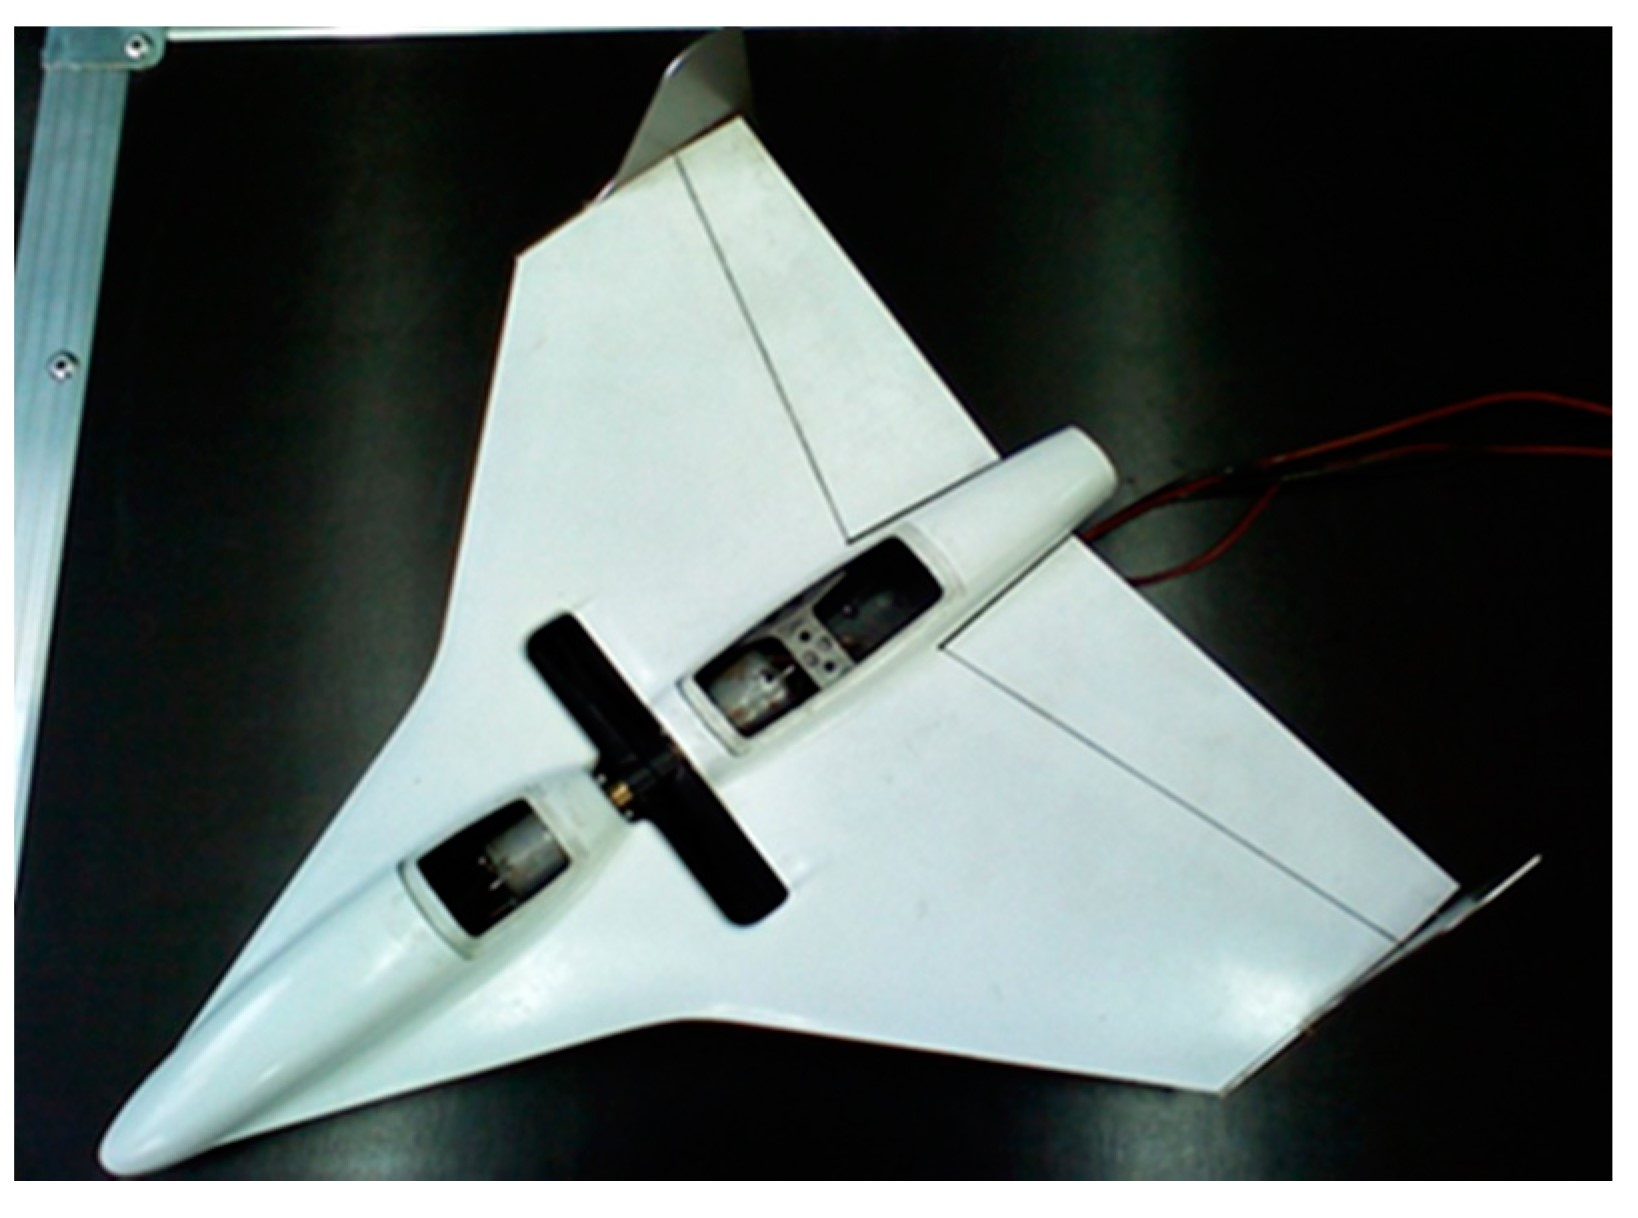
\includegraphics[width=\textwidth]{01_Introduction/Figs/fixed.jpg}
         \caption{Fixed wing MAV \cite{Sibilski2020}}
         %\label{fig:y equals x}
     \end{subfigure}
     \hfill
     \begin{subfigure}[b]{0.3\textwidth}
         \centering
         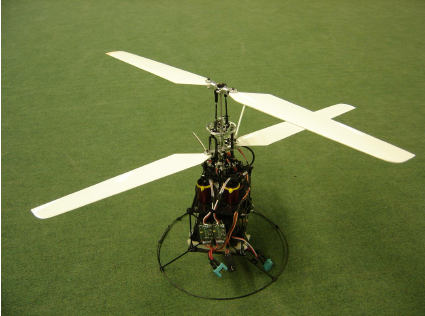
\includegraphics[width=\textwidth]{01_Introduction/Figs/rotar.png}
         \caption{Rotor MAV \cite{rotar2022}}
         %\label{fig:three sin x}
     \end{subfigure}
     \hfill
     \begin{subfigure}[b]{0.3\textwidth}
         \centering
         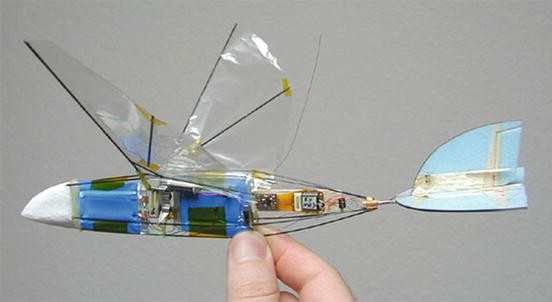
\includegraphics[width=\textwidth]{01_Introduction/Figs/flapping.jpg}
         \caption{Flapping wing MAV \cite{Jones2015}}
         %\label{fig:five over x}
     \end{subfigure}
        \caption{Examples of MAVs with category}
        \label{fig:threeDesigns}
\end{figure}


MAVs are much more difficult to design and manufacture than typical aircraft  \cite{Ward2017}. This additional complexity is due to several factors:
\begin{itemize}
  \item Low speed flight
  \item Small physical dimensions
  \item Structural strength
  \item Reduced stall speed due to smaller size
  \item Low inertia
\end{itemize}



% \\
With the increased complexity of MAV designs, there has also been an increased interest in the research and design of optimised MAV models \cite{Ward2017}. Design software to optimise MAV designs is generally based on aerodynamic properties, weights, stability, and maneuverability \cite{Amadori2012} \cite{Vijayanandh2019} \cite{Radmanesh2014}. The low-speed and non-linear flight dynamics are of particular importance for MAV development \cite{Aboelezz2020} \cite{Aboelezz2021}. The low speeds that MAVs fly at and the influence of an operating propeller on the rest of the MAV is currently unvalidated with physical wind tunnel testing. This thesis aims to fill in this gap.

% There is no physically validated MAV modelling  validated, reliable optimisation technique for MAV aircraft design.

% 

% Intro here




\section{Problem Statement}
\label{ProblemStatement}

In the past, surveillance was conducted initially from hot air balloons. Later, aircraft such as helicopters would be used, costing companies large sums of money to survey from a bird's eye view \cite{Aleksander2018}. Today drones and UAVs often conduct this work, within certain limits due to range and flight time \cite{NONAMI2007} \cite{Aleksander2018}. The next significant technology jump sees the optimisation and miniaturisation of these aircraft to produce MAVs. MAVs are set to increase the ability to conduct a variety of missions that predominately have military or surveillance objectives \cite{Aleksander2018} \cite{Mil2022} \cite{Greenwood2019} \cite{Saytov2022}. 

The MAV's main deferring attributes are; its smaller size, lower radar visibility and lower noise output. With MAV design becoming one of the fastest-growing areas of development in the aerospace industry, there is an increasing need to have accurate experimental data to validate, simulate and model the numerous MAV configurations being investigated. One of the core but currently missing pieces to this puzzle is the influence and effect of propellers on the aerodynamics and stability of MAVs. Can we further deepen our understanding of MAVs by analysing these effects?
% DEEPERRR

% paragraph on impact\significance of MAV
% MAV's

% paragraph on current Limitations


% paragraph on challenge/ main goal 
\section{Objectives}
\label{sec:Objectives}
The objectives of this thesis are as follows:

\begin{enumerate}
  \item To carry out a review of current published literature and determine areas with insufficient or no research available for further development and research.
  \item To design and produce a 3D model of a MAV with an interchanable propeller to allow for both tractor and pusher configurations.
  \item To conduct wind tunnel testing of the MAV model with and without propeller effects.
  \item To analyse data of wind tunnel results and detail the effect that propellers have on the MAV model.
\end{enumerate}

\section{Outline}
\label{sec:Outline}
An outline of the proposed final submission is listed below. However, it is subject to change.

\begin{itemize}
  \item Chapter 2: Background \newline This chapter outlines the core theory and relevant literature for understanding current MAV technology, provides information surrounding the key issues to be addressed and justifies the need for conducting this study. 
  \item Chapter 3: Literature Review \newline This chapter outlines the current information relating to MAVs and propeller effects. Previous studies and current literature is outlined here along with how this study will extend or differ from previous work.
  \item Chapter 4: Methodology \newline This chapter outlines the Methodology to develop the MAV model, complete wind tunnel testing and validate results using VAP 3.
  \item Chapter 5: Results \newline This chapter outlines the final results of the study and comapares these results with validation cases from VAP 3.
  \item Chapter 6: Discussion and Future Work \newline This chapter gives reasons for the results seen in the study and recommends future work to be investigated. 
\end{itemize}



% \begin{python}[caption=Example computation]
% // Calculate the multiplication of x and y by adding x, y number of times.
% function multiply(x, y):
%   output = 0

%   for i = 0..y:
%     output = output + x

%   return output
% \end{python}
